% ===========================================================================
%  TikuOS — Test Suite Architecture & Design
%  Beamer Presentation
% ===========================================================================
\documentclass[aspectratio=169, 10pt]{beamer}

% ---- Theme ----------------------------------------------------------------
\usetheme{Madrid}
\usecolortheme{whale}
\setbeamertemplate{navigation symbols}{}
\setbeamertemplate{footline}{%
  \leavevmode\hbox{%
    \begin{beamercolorbox}[wd=.33\paperwidth,ht=2.5ex,dp=1ex,center]{author in head/foot}%
      \usebeamerfont{author in head/foot}\insertshortauthor
    \end{beamercolorbox}%
    \begin{beamercolorbox}[wd=.34\paperwidth,ht=2.5ex,dp=1ex,center]{title in head/foot}%
      \usebeamerfont{title in head/foot}\insertshorttitle
    \end{beamercolorbox}%
    \begin{beamercolorbox}[wd=.33\paperwidth,ht=2.5ex,dp=1ex,right]{date in head/foot}%
      \usebeamerfont{date in head/foot}\insertshortdate{}\hspace*{2em}%
      \insertframenumber{}/\inserttotalframenumber\hspace*{2ex}
    \end{beamercolorbox}}%
  \vskip0pt%
}

% ---- Packages -------------------------------------------------------------
\usepackage{listings}
\usepackage{graphicx}
\usepackage{hyperref}
\usepackage{booktabs}
\usepackage{multirow}
\usepackage{tikz}
\usetikzlibrary{arrows.meta, positioning, shapes.geometric, calc, decorations.pathreplacing}

% ---- Code listing style ---------------------------------------------------
\lstset{
  basicstyle=\ttfamily\scriptsize,
  keywordstyle=\color{blue}\bfseries,
  commentstyle=\color{gray},
  stringstyle=\color{red!70!black},
  showstringspaces=false,
  breaklines=true,
  frame=single,
  rulecolor=\color{black!30},
  backgroundcolor=\color{blue!3},
  tabsize=4,
}
\lstdefinestyle{cstyle}{
  language=C,
  morekeywords={uint8_t,uint16_t,uint32_t,tiku_arena_t,tiku_mem_stats_t,
                tiku_mem_err_t,tiku_mem_arch_size_t,TIKU_MEM_OK,
                TIKU_MEM_ERR_INVALID,TIKU_MEM_ERR_NOMEM,NULL,
                TEST_ASSERT,TEST_SUITE_BEGIN,TEST_SUITE_END,
                TEST_GROUP_BEGIN,TEST_GROUP_END,TEST_PRINT,
                TEST_ENABLE,TIKU_PRINTF,PLATFORM_MSP430,
                HAS_TIKUKITS,TEST_KITS,TEST_KITS_MATRIX},
}
\lstdefinestyle{bashstyle}{
  language=bash,
  morekeywords={sudo,apt,make,gcc},
}
\lstdefinestyle{outputstyle}{
  basicstyle=\ttfamily\scriptsize\color{black!80},
  frame=single,
  rulecolor=\color{black!30},
  backgroundcolor=\color{green!3},
  breaklines=true,
}

% ---- Metadata -------------------------------------------------------------
\title[TikuOS Testing]{TikuOS Test Suite}
\subtitle{Simple. Ubiquitous. Intelligence, Everywhere.}
\author[Ambuj Varshney]{Ambuj Varshney \\ \texttt{ambuj@tiku-os.org}}
\date{\today}

% ===========================================================================
\begin{document}

% ---------------------------------------------------------------------------
\begin{frame}
\titlepage
\end{frame}

% ---------------------------------------------------------------------------
\begin{frame}{Outline}
\tableofcontents
\end{frame}

% ===========================================================================
\section{Why a Test Framework?}
% ===========================================================================

\begin{frame}{Testing on Bare-Metal MCUs is Hard}
\begin{columns}[T]
\begin{column}{0.48\textwidth}
\textbf{Challenges:}
\begin{itemize}
  \item No OS, no test runner, no \texttt{stdout}
  \item Tests must run on real hardware over UART
  \item Limited flash (48--256\,KB) and SRAM (2--8\,KB)
  \item Subsystems interact with ISRs, watchdogs, MPU
  \item Optional libraries (tikukits) may or may not be present
\end{itemize}

\vspace{0.5em}
\begin{alertblock}{No Standard Framework Fits}
Host-side test frameworks (CUnit, Unity) assume \texttt{malloc},
\texttt{printf}, and a hosted environment. TikuOS needs a
zero-overhead, UART-friendly harness.
\end{alertblock}
\end{column}

\begin{column}{0.48\textwidth}
\textbf{TikuOS Test Framework Goals:}
\begin{itemize}
  \item Single shared harness header
  \item Machine-parseable output over UART
  \item Human-readable at the same time
  \item Per-module enable flags (no wasted flash)
  \item Compile-time mutual exclusion
  \item Optional library integration (tikukits)
  \item Runs on-target \textbf{and} host-native
\end{itemize}

\vspace{0.5em}
\begin{block}{Key Insight}
Embed the test protocol \textbf{in the output format} itself ---
no host-side agent needed, just parse UART lines.
\end{block}
\end{column}
\end{columns}
\end{frame}

% ===========================================================================
\section{Architecture Overview}
% ===========================================================================

\begin{frame}{Test Framework Architecture}
\begin{center}
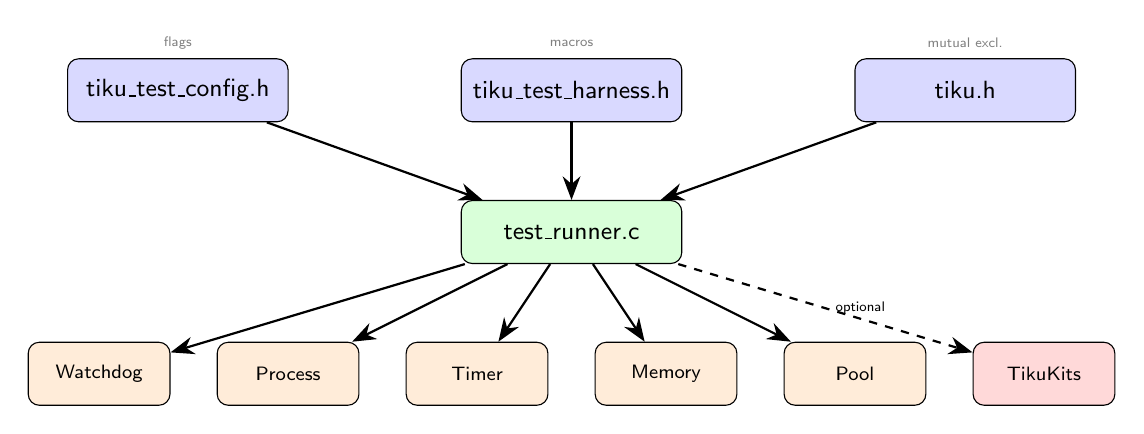
\begin{tikzpicture}[
    box/.style={draw, rounded corners, minimum width=2.8cm, minimum height=0.8cm,
                font=\small\sffamily, fill=#1},
    arr/.style={-{Stealth[length=3mm]}, thick},
    >=Stealth
  ]

  % Top level
  \node[box=blue!15] (config) at (0, 0) {tiku\_test\_config.h};
  \node[box=blue!15] (harness) at (5, 0) {tiku\_test\_harness.h};
  \node[box=blue!15] (tiku) at (10, 0) {tiku.h};

  % Middle level
  \node[box=green!15] (runner) at (5, -1.8) {test\_runner.c};

  % Bottom level - test modules
  \node[box=orange!15, minimum width=1.8cm] (watchdog) at (-1, -3.6) {\scriptsize Watchdog};
  \node[box=orange!15, minimum width=1.8cm] (process) at (1.4, -3.6) {\scriptsize Process};
  \node[box=orange!15, minimum width=1.8cm] (timer) at (3.8, -3.6) {\scriptsize Timer};
  \node[box=orange!15, minimum width=1.8cm] (memory) at (6.2, -3.6) {\scriptsize Memory};
  \node[box=orange!15, minimum width=1.8cm] (pool) at (8.6, -3.6) {\scriptsize Pool};
  \node[box=red!15, minimum width=1.8cm] (kits) at (11, -3.6) {\scriptsize TikuKits};

  % Arrows
  \draw[arr] (config) -- (runner);
  \draw[arr] (harness) -- (runner);
  \draw[arr] (tiku) -- (runner);
  \draw[arr] (runner) -- (watchdog);
  \draw[arr] (runner) -- (process);
  \draw[arr] (runner) -- (timer);
  \draw[arr] (runner) -- (memory);
  \draw[arr] (runner) -- (pool);
  \draw[arr, dashed] (runner) -- (kits)
    node[midway, right, font=\tiny\sffamily] {optional};

  % Labels
  \node[font=\tiny\sffamily, gray] at (0, 0.6) {flags};
  \node[font=\tiny\sffamily, gray] at (5, 0.6) {macros};
  \node[font=\tiny\sffamily, gray] at (10, 0.6) {mutual excl.};

\end{tikzpicture}
\end{center}

\vspace{0.5em}
\begin{block}{Three Header Layers}
\textbf{tiku\_test\_config.h} --- per-module enable flags \quad
\textbf{tiku\_test\_harness.h} --- assertion \& output macros \quad
\textbf{tiku.h} --- mutual exclusion guards
\end{block}
\end{frame}

% ---------------------------------------------------------------------------
\begin{frame}{Firmware Modes: Mutual Exclusion}
\begin{center}
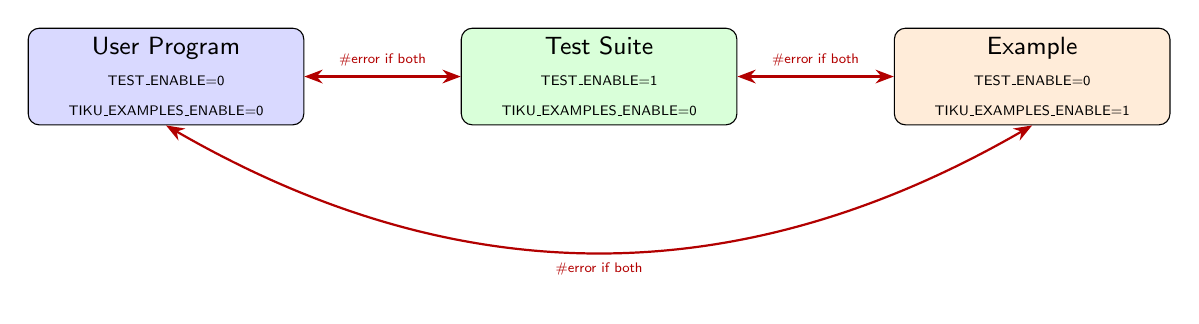
\begin{tikzpicture}[
    mode/.style={draw, rounded corners, minimum width=3.5cm, minimum height=1.2cm,
                 font=\small\sffamily, fill=#1, align=center},
    arr/.style={-{Stealth[length=3mm]}, thick, red!70!black},
    >=Stealth
  ]

  \node[mode=blue!15] (user) at (0, 0) {User Program\\{\tiny TEST\_ENABLE=0}\\{\tiny TIKU\_EXAMPLES\_ENABLE=0}};
  \node[mode=green!15] (test) at (5.5, 0) {Test Suite\\{\tiny TEST\_ENABLE=1}\\{\tiny TIKU\_EXAMPLES\_ENABLE=0}};
  \node[mode=orange!15] (example) at (11, 0) {Example\\{\tiny TEST\_ENABLE=0}\\{\tiny TIKU\_EXAMPLES\_ENABLE=1}};

  \draw[arr, <->] (user) -- (test) node[midway, above, font=\tiny\sffamily] {\#error if both};
  \draw[arr, <->] (test) -- (example) node[midway, above, font=\tiny\sffamily] {\#error if both};
  \draw[arr, <->] (user.south) to[bend right=30] node[midway, below, font=\tiny\sffamily] {\#error if both} (example.south);

\end{tikzpicture}
\end{center}

\vspace{0.3em}
\begin{columns}[T]
\begin{column}{0.48\textwidth}
\begin{lstlisting}[style=cstyle, title={tiku.h --- mode guard}]
#if TEST_ENABLE && TIKU_EXAMPLES_ENABLE
#error "TEST_ENABLE and "
  "TIKU_EXAMPLES_ENABLE "
  "cannot both be 1"
#endif
\end{lstlisting}
\end{column}

\begin{column}{0.48\textwidth}
\begin{block}{Three Firmware Modes}
Exactly \textbf{one} mode at compile time:
\begin{enumerate}
  \item \textbf{User program} --- production firmware
  \item \textbf{Test suite} --- one test category active
  \item \textbf{Example} --- one example demo active
\end{enumerate}
The compiler enforces this --- no runtime check needed.
\end{block}
\end{column}
\end{columns}
\end{frame}

% ---------------------------------------------------------------------------
\begin{frame}[fragile]{Test Category Mutual Exclusion}
\begin{lstlisting}[style=cstyle, title={tests/tiku\_test\_config.h --- only one category at a time}]
#define _TEST_CATEGORY_COUNT                                                 \
    (!!TEST_WATCHDOG + !!TEST_CPUCLOCK + !!TEST_PROCESS + !!TEST_TIMER +     \
     !!TEST_MEM + !!TEST_PERSIST + !!TEST_MPU + !!TEST_POOL +               \
     !!TEST_REGION + !!TEST_KITS_MATRIX + !!TEST_KITS_STATISTICS +          \
     !!TEST_KITS_DISTANCE + !!TEST_KITS_SENSOR + !!TEST_KITS_SIGFEATURES + \
     !!TEST_KITS_TEXTCOMPRESSION)

#if TEST_ENABLE && (_TEST_CATEGORY_COUNT > 1)
#error "Only one test category may be enabled at a time"
#endif
\end{lstlisting}

\vspace{0.3em}
\begin{block}{Why Only One Category?}
\begin{itemize}
  \item MCU flash is limited (48--256\,KB) --- including all test code would overflow
  \item Linker \texttt{-{}-gc-sections} eliminates dead code, but only if sections are truly unreferenced
  \item Some tests reinitialize subsystems (process, timer, watchdog) --- running two would conflict
  \item Compile-time \texttt{\#error} catches mistakes before flashing
\end{itemize}
\end{block}
\end{frame}

% ===========================================================================
\section{Test Harness}
% ===========================================================================

\begin{frame}[fragile]{Shared Test Harness: tiku\_test\_harness.h}
\begin{columns}[T]
\begin{column}{0.48\textwidth}
\begin{lstlisting}[style=cstyle, title={Platform-aware print}]
#ifdef PLATFORM_MSP430
#include "tiku.h"
#define TEST_PRINT(...) \
    TIKU_PRINTF(__VA_ARGS__)
#else
#define TEST_PRINT(...) \
    printf(__VA_ARGS__)
#endif
\end{lstlisting}

\begin{lstlisting}[style=cstyle, title={Global counters}]
extern int tests_run;
extern int tests_passed;
extern int tests_failed;
\end{lstlisting}

\vspace{0.3em}
\begin{block}{Single Source of Truth}
All test modules include this one header ---
no duplicate macro definitions across modules.
\end{block}
\end{column}

\begin{column}{0.48\textwidth}
\begin{lstlisting}[style=cstyle, title={Assertion macro}]
#define TEST_ASSERT(cond, msg)      \
  do {                              \
    tests_run++;                    \
    if (cond) {                     \
      tests_passed++;               \
      TEST_PRINT(                   \
        "[T:P:%d] %s\n",           \
        tests_run, msg);            \
    } else {                        \
      tests_failed++;               \
      TEST_PRINT(                   \
        "[T:F:%d] %s\n",           \
        tests_run, msg);            \
    }                               \
  } while (0)
\end{lstlisting}

\vspace{0.3em}
\begin{alertblock}{No \texttt{abort()} or \texttt{exit()}}
On an MCU, there is nowhere to exit \emph{to}.
Every assertion runs --- no early termination.
\end{alertblock}
\end{column}
\end{columns}
\end{frame}

% ---------------------------------------------------------------------------
\begin{frame}[fragile]{Suite and Group Markers}
\begin{lstlisting}[style=cstyle, title={Suite markers --- bracket the entire test run}]
#define TEST_SUITE_BEGIN(name)                                               \
    do {                                                                     \
        tests_run    = 0;                                                    \
        tests_passed = 0;                                                    \
        tests_failed = 0;                                                    \
        TEST_PRINT("[TS:BEGIN] %s\n", name);                                \
    } while (0)

#define TEST_SUITE_END(name)                                                 \
    TEST_PRINT("[TS:END] %s total=%d pass=%d fail=%d\n",                    \
               name, tests_run, tests_passed, tests_failed)
\end{lstlisting}

\begin{lstlisting}[style=cstyle, title={Group markers --- bracket a logical test function}]
#define TEST_GROUP_BEGIN(name)   TEST_PRINT("[TG:BEGIN] %s\n", name)
#define TEST_GROUP_END(name)    TEST_PRINT("[TG:END] %s\n", name)
\end{lstlisting}

\vspace{0.3em}
\begin{block}{Three-Level Hierarchy}
\textbf{Suite} $\supset$ \textbf{Group} $\supset$ \textbf{Assertion} ---
suites reset counters, groups organize related assertions,
and each assertion emits a pass/fail tag.
\end{block}
\end{frame}

% ===========================================================================
\section{Output Format}
% ===========================================================================

\begin{frame}[fragile]{Machine-Parseable Output Protocol}
\begin{table}
\centering
\small
\begin{tabular}{@{}llp{7.5cm}@{}}
\toprule
\textbf{Tag} & \textbf{Direction} & \textbf{Meaning} \\
\midrule
\texttt{[TS:BEGIN] name}  & Start & Test suite started; counters reset to zero \\
\texttt{[TG:BEGIN] name}  & Start & Test group (logical function) started \\
\texttt{[T:P:N] msg}      & Result & Assertion \texttt{N} \textbf{passed} \\
\texttt{[T:F:N] msg}      & Result & Assertion \texttt{N} \textbf{failed} \\
\texttt{[TG:END] name}    & End & Test group ended \\
\texttt{[TS:END] name total=T pass=P fail=F} & End & Suite summary \\
\bottomrule
\end{tabular}
\end{table}

\vspace{0.3em}
\begin{block}{Design Choices}
\begin{itemize}
  \item Square-bracket tags are easy to \texttt{grep} from mixed UART output
  \item \texttt{N} is a monotonically increasing counter --- detects dropped lines
  \item The \texttt{[TS:END]} line is self-contained: a single regex extracts total/pass/fail
  \item Human-readable \emph{and} machine-parseable --- no separate verbose/quiet modes
\end{itemize}
\end{block}
\end{frame}

% ---------------------------------------------------------------------------
\begin{frame}[fragile]{Example UART Output}
\begin{lstlisting}[style=outputstyle, title={Captured from MSP430FR5969 over UART @ 115200 baud}]
[TS:BEGIN] TikuOS
[TG:BEGIN] Matrix Init
[T:P:1] init 2x3 returns OK
[T:P:2] rows == 2
[T:P:3] cols == 3
[T:P:4] all elements zero after init
[TG:END] Matrix Init
[TG:BEGIN] Matrix Identity
[T:P:5] identity 3x3 returns OK
[T:P:6] diagonal elements are 1.0
[T:P:7] off-diagonal elements are 0.0
[TG:END] Matrix Identity
  ...
[TG:BEGIN] Matrix Null Inputs
[T:P:110] null matrix rejected
[T:P:111] null data buffer rejected
[T:P:112] zero rows rejected
[TG:END] Matrix Null Inputs
[TS:END] TikuOS total=112 pass=112 fail=0
\end{lstlisting}

\vspace{0.3em}
\begin{block}{Parsing the Summary}
A CI script only needs: \texttt{grep '\textasciicircum\textbackslash[TS:END\textbackslash]'} $\rightarrow$ extract \texttt{fail=N} $\rightarrow$ exit code.
\end{block}
\end{frame}

% ---------------------------------------------------------------------------
\begin{frame}[fragile]{Parsing for Automated Testing}
\begin{columns}[T]
\begin{column}{0.48\textwidth}
\begin{lstlisting}[style=bashstyle, title={Shell: check pass/fail}]
# Capture UART output to file
make monitor > uart.log &
sleep 10 && kill %1

# Extract summary line
SUMMARY=$(grep '^\[TS:END\]' uart.log)

# Parse fail count
FAIL=$(echo "$SUMMARY" | \
  sed 's/.*fail=\([0-9]*\)/\1/')

if [ "$FAIL" -ne 0 ]; then
  echo "FAILED: $FAIL assertions"
  exit 1
fi
echo "ALL TESTS PASSED"
\end{lstlisting}
\end{column}

\begin{column}{0.48\textwidth}
\begin{lstlisting}[language=Python, style=cstyle, title={Python: parse all results}]
import re

with open("uart.log") as f:
    for line in f:
        m = re.match(
            r'\[T:([PF]):(\d+)\] (.+)',
            line)
        if m:
            status = m.group(1)
            num    = int(m.group(2))
            msg    = m.group(3)
            print(f"{'PASS' if status=='P'"
                  f" else 'FAIL'}"
                  f" #{num}: {msg}")
\end{lstlisting}

\vspace{0.3em}
\begin{block}{Extensible}
The tagged format supports future tooling: dashboards,
regression databases, or diff-based failure analysis.
\end{block}
\end{column}
\end{columns}
\end{frame}

% ===========================================================================
\section{Test Categories}
% ===========================================================================

\begin{frame}{Core OS Test Modules}
\begin{table}
\centering
\small
\begin{tabular}{@{}llrl@{}}
\toprule
\textbf{Module} & \textbf{Config Flag} & \textbf{Tests} & \textbf{Covers} \\
\midrule
Watchdog    & \texttt{TEST\_WATCHDOG}  & 4  & kick, pause/resume, interval, timeout \\
Process     & \texttt{TEST\_PROCESS}   & 10 & lifecycle, events, yield, broadcast, poll, queue, local storage \\
Timer       & \texttt{TEST\_TIMER}     & 6  & event, callback, periodic, stop, hardware timer \\
Arena       & \texttt{TEST\_MEM}       & 9  & create, alloc, alignment, full, reset, peak, secure wipe \\
Pool        & \texttt{TEST\_POOL}      & 14 & create, alloc/free, exhaustion, LIFO, peak, poisoning \\
Persist     & \texttt{TEST\_PERSIST}   & 12 & init, register, read/write, delete, reboot, wear \\
MPU         & \texttt{TEST\_MPU}       & 11 & init, lock/unlock, permissions, scoped write, violations \\
Region      & \texttt{TEST\_REGION}    & 12 & init, contains, boundary, overflow, claim/unclaim \\
CPU Clock   & \texttt{TEST\_CPUCLOCK}  & 1  & clock output pin for oscilloscope verification \\
\bottomrule
\end{tabular}
\end{table}

\vspace{0.3em}
\begin{block}{79 Core OS Tests}
Each module has its own header, source file(s), and fine-grained sub-flags.
Auto-derived flags (\texttt{TEST\_MEM}, \texttt{TEST\_PROCESS}, etc.)
aggregate sub-flags via \texttt{||} expressions.
\end{block}
\end{frame}

% ---------------------------------------------------------------------------
\begin{frame}{TikuKits Library Tests}
\begin{table}
\centering
\small
\begin{tabular}{@{}llrl@{}}
\toprule
\textbf{Module} & \textbf{Config Flag} & \textbf{Functions} & \textbf{Covers} \\
\midrule
Matrix       & \texttt{TEST\_KITS\_MATRIX}       & 12 & init, identity, get/set, add/sub, mul, scale, det, trace \\
Statistics   & \texttt{TEST\_KITS\_STATISTICS}    & 8  & windowed, Welford, min/max, EWMA, energy, isqrt \\
Distance     & \texttt{TEST\_KITS\_DISTANCE}      & 6  & Manhattan, Euclidean, dot, cosine, Hamming \\
Sensor       & \texttt{TEST\_KITS\_SENSOR}        & 2  & fractional conversion, sensor name lookup \\
Sig.\ Features & \texttt{TEST\_KITS\_SIGFEATURES} & 8  & peak, ZCR, histogram, delta, Goertzel, z-score, scale \\
Compression  & \texttt{TEST\_KITS\_TEXTCOMPRESSION} & 4 & RLE, byte-pair, heatshrink round-trip \\
\bottomrule
\end{tabular}
\end{table}

\vspace{0.3em}
\begin{alertblock}{TikuKits is Optional}
All tikukits test flags are guarded by \texttt{\#if defined(HAS\_TIKUKITS)}.
When the \texttt{tikukits/} directory is absent, all flags default to~0
and the compiler never sees tikukits headers or sources.
\end{alertblock}
\end{frame}

% ===========================================================================
\section{TikuKits Integration}
% ===========================================================================

\begin{frame}[fragile]{Optional Library Detection}
\begin{center}
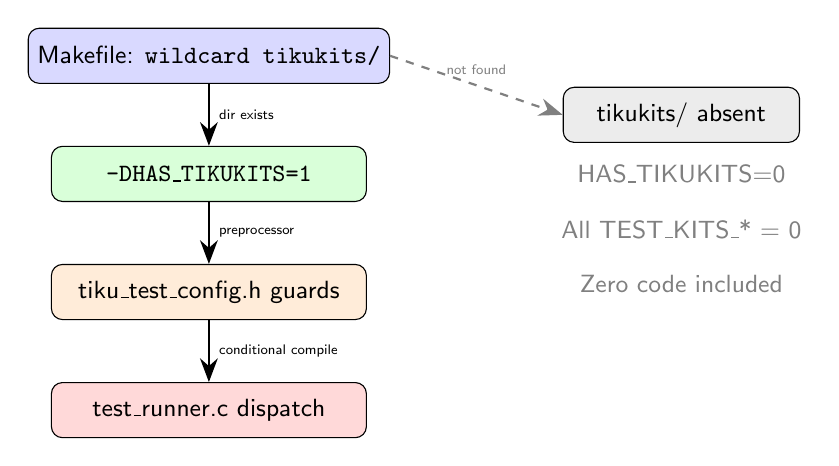
\begin{tikzpicture}[
    step/.style={draw, rounded corners, minimum width=4cm, minimum height=0.7cm,
                 font=\small\sffamily, fill=#1},
    arr/.style={-{Stealth[length=3mm]}, thick},
    >=Stealth
  ]

  \node[step=blue!15] (makefile) at (0, 0) {Makefile: \texttt{wildcard tikukits/}};
  \node[step=green!15] (cflag) at (0, -1.5) {\texttt{-DHAS\_TIKUKITS=1}};
  \node[step=orange!15] (config) at (0, -3.0) {tiku\_test\_config.h guards};
  \node[step=red!15] (runner) at (0, -4.5) {test\_runner.c dispatch};

  \draw[arr] (makefile) -- (cflag) node[midway, right, font=\tiny\sffamily] {dir exists};
  \draw[arr] (cflag) -- (config) node[midway, right, font=\tiny\sffamily] {preprocessor};
  \draw[arr] (config) -- (runner) node[midway, right, font=\tiny\sffamily] {conditional compile};

  % "not present" path
  \node[step=gray!15, minimum width=3cm] (absent) at (6, -0.75) {tikukits/ absent};
  \draw[arr, dashed, gray] (makefile.east) -- (absent.west)
    node[midway, above, font=\tiny\sffamily] {not found};
  \node[font=\small\sffamily, gray] at (6, -1.5) {HAS\_TIKUKITS=0};
  \node[font=\small\sffamily, gray] at (6, -2.2) {All TEST\_KITS\_* = 0};
  \node[font=\small\sffamily, gray] at (6, -2.9) {Zero code included};

\end{tikzpicture}
\end{center}

\vspace{0.3em}
\begin{block}{Guard Chain}
Makefile auto-detects $\rightarrow$ sets \texttt{-D} flag $\rightarrow$ config header
enables/disables flags $\rightarrow$ test runner conditionally compiles.
TikuOS always builds independently.
\end{block}
\end{frame}

% ---------------------------------------------------------------------------
\begin{frame}[fragile]{Makefile: Conditional Source Inclusion}
\begin{lstlisting}[style=bashstyle, title={Makefile --- tikukits sources (library + tests)}]
HAS_TIKUKITS := $(if $(wildcard $(PROJ_DIR)/tikukits),1,0)
ifeq ($(HAS_TIKUKITS),1)
CFLAGS += -DHAS_TIKUKITS=1

# Library sources (only modules actually used get linked)
SRCS += $(wildcard tikukits/maths/linear_algebra/*.c)
SRCS += $(wildcard tikukits/maths/statistics/*.c)
SRCS += $(wildcard tikukits/maths/distance/*.c)
SRCS += $(wildcard tikukits/sensors/temperature/*.c)
SRCS += $(wildcard tikukits/sigfeatures/*/*.c)
SRCS += $(wildcard tikukits/textcompression/*/*.c)

# Test sources (only when testing is enabled)
ifeq ($(HAS_TESTS),1)
SRCS += $(wildcard tikukits/tests/maths/*.c)
SRCS += $(wildcard tikukits/tests/sensors/*.c)
SRCS += $(wildcard tikukits/tests/sigfeatures/*.c)
SRCS += $(wildcard tikukits/tests/textcompression/*.c)
endif
endif
\end{lstlisting}

\vspace{0.3em}
\begin{block}{Dead Code Elimination}
\texttt{-ffunction-sections -fdata-sections} + \texttt{-Wl,-{}-gc-sections}
ensures unused library functions are stripped from the final binary.
\end{block}
\end{frame}

% ===========================================================================
\section{Configuration \& Running Tests}
% ===========================================================================

\begin{frame}[fragile]{Enabling a Test}
\begin{columns}[T]
\begin{column}{0.48\textwidth}
\begin{lstlisting}[style=cstyle, title={tests/tiku\_test\_config.h}]
/* Step 1: Enable master switch */
#define TEST_ENABLE 1

/* Step 2: Enable ONE category */
#define TEST_KITS_MATRIX 1

/* All others stay 0 */
#define TEST_WATCHDOG 0
#define TEST_PROCESS_LIFECYCLE 0
#define TEST_MEM_CREATE 0
/* ... */
\end{lstlisting}

\vspace{0.3em}
\begin{alertblock}{Common Mistake}
Forgetting \texttt{TEST\_ENABLE = 1} --- the category
flag alone is not enough. The master switch gates
\texttt{test\_run\_all()} in \texttt{main()}.
\end{alertblock}
\end{column}

\begin{column}{0.48\textwidth}
\begin{lstlisting}[style=bashstyle, title={Build, flash, and monitor}]
# Build for MSP430FR5969
make clean
make MCU=msp430fr5969

# Flash via MSP-FET programmer
make flash MCU=msp430fr5969

# Monitor UART output
make monitor
\end{lstlisting}

\vspace{0.5em}
\begin{block}{Auto-Derived Flags}
You only set leaf flags (\texttt{TEST\_MEM\_CREATE},
\texttt{TEST\_KITS\_MATRIX}). Parent flags are computed
automatically via \texttt{||} expressions:
\begin{itemize}
  \item \texttt{TEST\_MEM} = OR of all arena sub-flags
  \item \texttt{TEST\_KITS\_MATHS} = matrix $|$ statistics $|$ distance
  \item \texttt{TEST\_KITS} = maths $|$ sensor $|$ sigfeatures $|$ textcomp
\end{itemize}
\end{block}
\end{column}
\end{columns}
\end{frame}

% ---------------------------------------------------------------------------
\begin{frame}[fragile]{Test Runner Dispatch}
\begin{lstlisting}[style=cstyle, title={tests/test\_runner.c --- main dispatch}]
void test_run_all(void)
{
    TEST_SUITE_BEGIN("TikuOS");

    /* Pre-interrupt tests */
    test_run_cpuclock();
    test_run_watchdog();
    test_run_process();
    test_run_mem();
    test_run_mpu();
    test_run_persist();
    test_run_pool();
    test_run_region();

    /* TikuKits library tests (no ISR dependency) */
#if defined(HAS_TIKUKITS)
    test_run_kits();
#endif

    /* Enable global interrupts (needed for timer ISRs) */
    __enable_interrupt();

    /* Post-interrupt tests */
    test_run_timer();

    TEST_SUITE_END("TikuOS");
}
\end{lstlisting}
\end{frame}

% ---------------------------------------------------------------------------
\begin{frame}[fragile]{Writing a New Test}
\begin{lstlisting}[style=cstyle, title={Example: a typical test function}]
#include "tests/tiku_test_harness.h"

void test_my_feature(void)
{
    TEST_GROUP_BEGIN("My Feature");

    /* Setup */
    int result = my_function(42);

    /* Assertions -- each emits a tagged UART line */
    TEST_ASSERT(result == 84,
                "my_function doubles its input");
    TEST_ASSERT(my_function(0) == 0,
                "my_function handles zero");
    TEST_ASSERT(my_function(-1) == -2,
                "my_function handles negative");

    TEST_GROUP_END("My Feature");
}
\end{lstlisting}

\vspace{0.3em}
\begin{block}{Convention}
One \texttt{TEST\_GROUP\_BEGIN/END} per function. Each \texttt{TEST\_ASSERT}
auto-increments the global counter and emits a \texttt{[T:P:N]} or \texttt{[T:F:N]} tag.
\end{block}
\end{frame}

% ===========================================================================
\section{Host-Native Testing}
% ===========================================================================

\begin{frame}[fragile]{Running Tests Without Hardware}
\begin{columns}[T]
\begin{column}{0.48\textwidth}
\begin{lstlisting}[style=bashstyle, title={Compile and run on host}]
gcc -std=c99 -Wall -Wextra -I. \
  tests/memory/test_mem_common.c \
  tests/memory/test_mem_arena.c \
  kernel/memory/tiku_mem.c \
  -o test_tiku_mem \
  && ./test_tiku_mem
\end{lstlisting}

\vspace{0.3em}
\begin{block}{Host Stubs}
\texttt{test\_mem\_common.c} provides:
\begin{itemize}
  \item \texttt{tiku\_mem\_arch\_init()} --- no-op
  \item \texttt{tiku\_mem\_arch\_secure\_wipe()} --- volatile loop
  \item \texttt{tiku\_mem\_arch\_nvm\_read/write()} --- \texttt{memcpy}
  \item Region table with test pools
  \item MPU register stubs
  \item \texttt{main()} that calls all tests
\end{itemize}
\end{block}
\end{column}

\begin{column}{0.48\textwidth}
\begin{lstlisting}[style=cstyle, title={Platform detection}]
#ifdef PLATFORM_MSP430
/* Real hardware paths */
#define TEST_PRINT(...) \
    TIKU_PRINTF(__VA_ARGS__)
#else
/* Host: plain printf */
#define TEST_PRINT(...) \
    printf(__VA_ARGS__)
#endif
\end{lstlisting}

\vspace{0.3em}
\begin{alertblock}{Same Assertions, Same Output}
The \textbf{exact same} \texttt{TEST\_ASSERT} macro runs
on both host and target. Output format is identical ---
the same parser works for both.
\end{alertblock}

\vspace{0.3em}
\begin{block}{What Can Run on Host}
Memory module tests (arena, pool, region, persist, MPU)
have full host stubs. Process, timer, and watchdog tests
require real MSP430 hardware.
\end{block}
\end{column}
\end{columns}
\end{frame}

% ===========================================================================
\section{File Organization}
% ===========================================================================

\begin{frame}[fragile]{Test Framework Files}
\begin{table}
\centering
\small
\begin{tabular}{@{}lll@{}}
\toprule
\textbf{Layer} & \textbf{File} & \textbf{Role} \\
\midrule
\multirow{3}{*}{Framework}
  & \texttt{tests/tiku\_test\_config.h}    & Per-module enable flags, mutual exclusion \\
  & \texttt{tests/tiku\_test\_harness.h}   & Assertion \& output macros \\
  & \texttt{tests/test\_runner.c}          & Central dispatch \\
\midrule
\multirow{4}{*}{Core OS Tests}
  & \texttt{tests/watchdog/*.c}    & Watchdog timer tests (4 files) \\
  & \texttt{tests/process/*.c}     & Process/protothread tests (10 files) \\
  & \texttt{tests/timer/*.c}       & Timer subsystem tests (6 files) \\
  & \texttt{tests/memory/*.c}      & Arena, pool, persist, MPU, region (5 files) \\
\midrule
\multirow{4}{*}{TikuKits Tests}
  & \texttt{tikukits/tests/maths/*.c}          & Matrix, statistics, distance \\
  & \texttt{tikukits/tests/sensors/*.c}        & Sensor interface \\
  & \texttt{tikukits/tests/sigfeatures/*.c}    & Signal feature extraction \\
  & \texttt{tikukits/tests/textcompression/*.c} & RLE, BPE, heatshrink \\
\midrule
Guards
  & \texttt{tiku.h}                         & Tests vs examples mutual exclusion \\
  & \texttt{examples/tiku\_example\_config.h} & Single-example guard \\
\bottomrule
\end{tabular}
\end{table}
\end{frame}

% ===========================================================================
\section{Summary}
% ===========================================================================

\begin{frame}{Summary}
\begin{columns}[T]
\begin{column}{0.48\textwidth}
\begin{block}{Test Framework Design}
\begin{itemize}
  \item Shared harness: \texttt{tiku\_test\_harness.h}
  \item Machine-parseable UART output
  \item Three-level hierarchy: suite $\supset$ group $\supset$ assertion
  \item Per-module compile-time enable flags
  \item Auto-derived parent flags via \texttt{||}
  \item Compile-time mutual exclusion (\texttt{\#error})
  \item Runs on-target and host-native
\end{itemize}
\end{block}

\vspace{0.3em}
\begin{block}{Output Protocol}
\texttt{[TS:BEGIN/END]}, \texttt{[TG:BEGIN/END]}, \texttt{[T:P/F:N]} ---
grep-friendly, counter-monotonic, self-contained summary line.
\end{block}
\end{column}

\begin{column}{0.48\textwidth}
\begin{block}{Test Coverage}
\begin{itemize}
  \item \textbf{79} core OS test assertions across 9 modules
  \item \textbf{40} tikukits test functions across 6 modules
  \item Watchdog, process, timer, memory, pool, persist, MPU, region
  \item Matrix, statistics, distance, sensor, signal features, compression
\end{itemize}
\end{block}

\vspace{0.3em}
\begin{alertblock}{TikuKits: Fully Optional}
Guard chain (Makefile $\rightarrow$ \texttt{-D} flag $\rightarrow$ \texttt{\#if} $\rightarrow$
conditional compile) ensures TikuOS builds and tests independently.
Zero tikukits code is included when the library is absent.
\end{alertblock}
\end{column}
\end{columns}
\end{frame}

% ---------------------------------------------------------------------------
\begin{frame}{Thank You}
\begin{center}
\Large\textbf{TikuOS Test Suite}\\[0.5em]
\normalsize Testing Framework for Physical AI Endpoints\\[1.5em]

\begin{tabular}{rl}
  Repository: & \url{https://github.com/tikuos/tikuOS} \\
  License:    & Apache 2.0 \\
  Harness:    & \texttt{tests/tiku\_test\_harness.h} \\
  Config:     & \texttt{tests/tiku\_test\_config.h} \\
  Runner:     & \texttt{tests/test\_runner.c} \\
\end{tabular}
\end{center}
\end{frame}

\end{document}
